\documentclass{article}
\usepackage{graphicx}
\usepackage[left=2cm, right=2cm, top=2cm]{geometry}
\usepackage{wrapfig}

\begin{document}
\centerline{\Large{\textbf{Swaraj Kaondal}}}
\noindent\rule{\textwidth}{1pt}\\
F-006, Hrushikesh,\hfill
Contact:\hspace{0.8cm} +91-99201368721     \\
Swami Samarth Nagar,\hfill
e-mailid:swarajkaon@gmail.com\\
Lokhandwala,\\
Andheri-West,\\
Mumbai-400053.
\begin{figure}[h]
\hfill
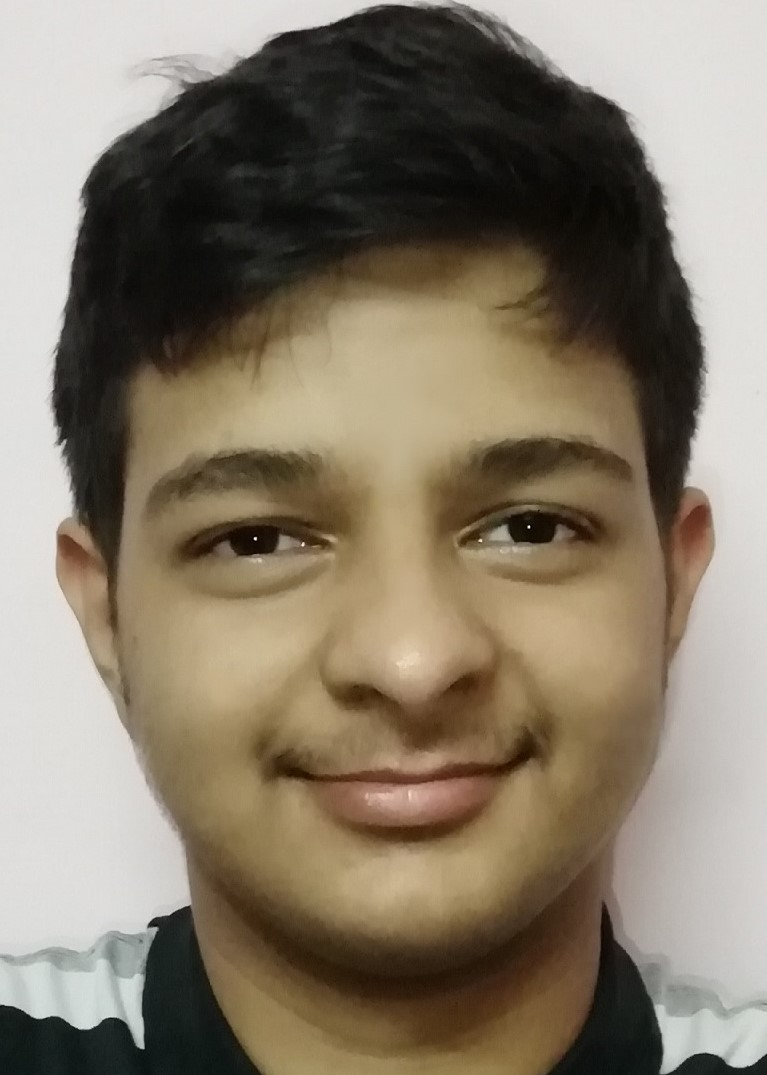
\includegraphics[scale = 0.08]{Swaraj.jpg}
\end{figure}
\section*{\textbf{CAREER OBJECTIVE}}
\noindent To have expert knowledge in Embedded Systems and be able to work in one of the top companies dealing with Embedded Systems.

\section*{\textbf{EDUCATION}}
\begin{tabular}{|c|c|c|c|c|}
\hline
Degree & College/School & University & Passing year & Pass percentage\\
\hline
SSC & Gyan Kendra High School & Maharashtra State Board & 2015 & 93.2\%\\
\hline
HSC & Hansraj Morarji College of Science & Maharashtra State Board & 2017 & 86.15\%\\
\hline
B.Tech & Sardar Patel Institute& Autonomous affliated  & - & -\\
 & of Technology & to Mumbai University & & \\
\hline 
\end{tabular}


\section*{\textbf{PROJECTS}}
\begin{itemize}
\item Line following bot using Arduino.
\item Pulse rate sensor using Arduino.
\end{itemize}

\section*{\textbf{TRAINING AND INTERNSHIP}}
\begin{itemize}
\item Recieved training in embeded systems by SafeTTy systems.
\end{itemize}


\section*{\textbf{RESEARCH PUBLICATIONS}}
-

\section*{\textbf{TECHNICAL SKILLS}}
\begin{itemize}
\item C.
\item Python (OpenCv, OpenGL).
\item Embedded C (Time triggered systems, Co-operative and hybrid schedulers).
\item IoT using MQTT protocol.
\item Autocad.
\end{itemize}


\section*{\textbf{SOFT SKILLS}}
\begin{itemize}
\item Good communication.
\item Adaptability.
\item Teamwork.
\end{itemize}
\end{document}